
Maxima is at heart a command line program, and by itself it is not
capable of displaying formatted mathematics beyond the ascii text
level. However there are other interfaces which may be used. Maxima
has the ability to export expressions using the \TeX{} syntax, and
several programs use this device to help with output formatting. (None
at this time allow formatted input.) All have their strengths and
weaknesses - the choice will likely depend on the skill of the user
and the task at hand. We will discuss here all of the interfaces currently
available, and the user can make the choice him/herself which one
to use. 


\section{The Terminal Interface}

~

{\centering 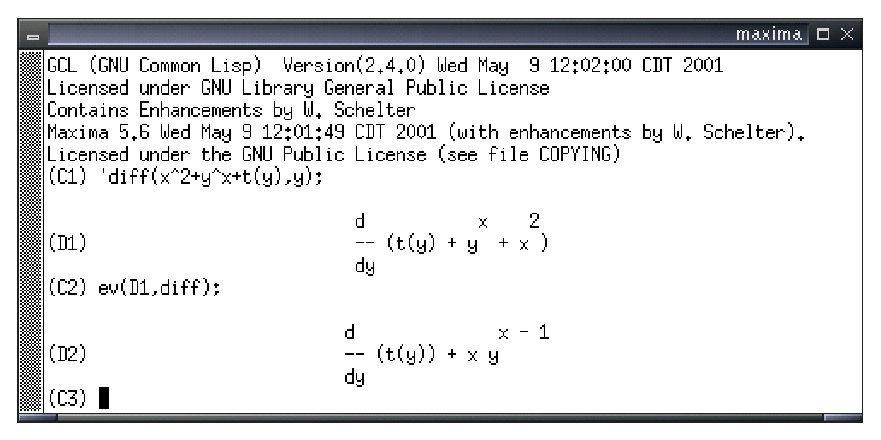
\includegraphics{images/terminalshot} \par }

~

The terminal interface is the original interface to Maxima. While
in some sense all of the interfaces to Maxima could be termed Terminal
interfaces, when we refer to it here we mean the command line, no
frills interface you would use in an xterm or a nongraphical terminal.
It is the least capable of all the alternatives in many respects,
but it is also the least demanding. 

How comfortable this interface is depends to a large extent on what
Lisp you used to compile Maxima originally. If you used the default,
which is gcl, (what all binary packages I am aware of use) you do
not have readline support on the terminal. This means you will not
be able to use the back arrow key to go to the middle of an expression
and change it - you must erase everything as you go back. This is
a serious limitation, and if this is the case it is recommended by
the author that you either compile against a Lisp flavor such as Clisp,
which has readline support, or use one of the other interfaces. Any
of the others should solve this problem. If you choose to use this
interface, you activate it by simply typing \texttt{maxima} on the
terminal prompt. 

The only times I'd really recommend this interface are when none of
the other options are viable, such as a telnet connection from a really
primitive terminal.  The other options, especially
the Emacs mode, are far more comfortable working environments. 

\section{The Emacs Interface}

A really excellent Emacs mode has been written for Maxima, and this is probably the
choice I would recommend instead of the bare terminal, with or without
a graphical interface. You get to
go back in an expression without having to erase your expression,
and in a graphical environment you get syntax highlighting, among many other
goodies.  There is also an environment for including Maxima input in LaTeX
documents.

\subsection{Installing the Maxima Emacs Mode}

\noindent
The Emaxima package consists of the files \texttt{maxima.el},
\texttt{emaxima.el}, \texttt{maxima-symbols.el},
\texttt{maxima-font-lock.el}, \texttt{emaxima.sty} and \texttt{emaxima.lisp}.
To install, place the \texttt{.el} files, as well as
\texttt{emaxima.lisp}\footnote{If Emacs cannot find
  \texttt{emaxima.lisp}, then the \TeX{} output functions will not
  work, any attempts to get \TeX{} output will only result in standard
  output.} 
somewhere in the load path for Emacs.
Finally, if you want to run \LaTeX{} on the resulting document, put
\texttt{emaxima.sty} somewhere in the \TeX{} inputs path.  If you use
pdflatex, you'll also need \texttt{pdfcolmk.sty}.

Although AucTeX is not strictly necessary, you will most likely find it worth
you time to install it, as many of the best features of Emaxima are LaTeX
oriented.  

Copy the \texttt{.el} and \texttt{.lisp} files to the site-lisp directory of your Emacs installation.
On a Redhat Linux system, for example, this would be /usr/share/emacs/site-lisp,
/usr/local/share/emacs/site-lisp, or some variation thereof.  Copy the \texttt{.sty}
files to a directory where LaTeX can see them - I've found on Redhat Linux
/usr/share/texmf/tex/latex/emaxima works fairly well.  Once you have done this,
run the command mktexlsr.  You should now be almost ready to roll.

The last step is to edit your .emacs file.  In order to use the enhanced terminal
mode, insert the following line:
\begin{verbatim}
(autoload 'maxima "maxima" "Maxima interaction" t)
\end{verbatim}
If you wish to associate files ending in \texttt{.max} with this particular
Emacs mode, add this line:
\begin{verbatim}
(setq auto-mode-alist (cons '("\\.max" . maxima-mode) auto-mode-alist)
\end{verbatim}
This will allow you to start Maxima from within Emacs.  You can do this
one of two ways - either start Emacs and from within it type \texttt{M-x maxima},
or from the command line type \texttt{emacs -f maxima} to have the whole thing
work in one step.  If you wish to create a desktop icon to start the command
line Maxima, simply place this line where they ask you what the name of your
program or executable is, and it should work quite smoothly.

For Maxima-mode, add the following line to .emacs:
\begin{verbatim}
(autoload 'maxima-mode "maxima" "Maxima mode" t)
\end{verbatim}
The command \texttt{M-x maxima-mode} will start you off here.

In the case of Emaxima, the line 
\begin{verbatim}
(autoload 'emaxima-mode "emaxima" "EMaxima" t)
\end{verbatim}
\noindent
should be inserted into your .emacs file.  Then typing
\texttt{M-x emaxima-mode} will start Emaxima mode.  The command 
\texttt{M-x emaxima-mark-file-as-emaxima} will put the line
\begin{verbatim}
%-*-EMaxima-*-
\end{verbatim}
\noindent
at the beginning of the file, if it isn't there already, and will ensure
that the next time the file is opened, it will be in \texttt{emaxima-mode}.  
This can be done automatically everytime a file is put in
\texttt{emaxima-mode} by putting the line
\begin{verbatim}
(add-hook 'emaxima-mode-hook 'emaxima-mark-file-as-emaxima)
\end{verbatim}
\noindent
somewhere in your \texttt{.emacs} file.


\subsection{Maxima-mode}

This mode is fairly basic, and is not dependant on LaTeX.  It basically amounts
to a text editor which allows you to send lines to Maxima.  

For moving around in the code, Maxima mode provides the following

\noindent
Maxima mode has the following completions commands:

\textbf{Motion}

\smallskip

\noindent
\begin{tabular}{p{\firstcol}p{\secondcol}}
\hline
\textbf{Key} & \textbf{Description}\\
\hline
\texttt{M-C-a} & Go to the beginning of the form.\\
\texttt{M-C-e} & Go to the end of the form.\\
\texttt{M-C-b} & Go to the beginning of the sexp.\\
\texttt{M-C-f} & Go to the end of the sexp.
\end{tabular}

\smallskip

\noindent
\textbf{Process}

\smallskip

\noindent
\begin{tabular}{p{\firstcol}p{\secondcol}}
\hline
\textbf{Key} & \textbf{Description}\\
\hline
\texttt{C-cC-p} & Start a Maxima process.\\
\texttt{C-cC-r} & Send the region to the Maxima process.\\
\texttt{C-cC-b} & Send the buffer to the Maxima process.\\
\texttt{C-cC-c} & Send the line to the Maxima process.\\
\texttt{C-cC-e} & Send the form to the Maxima process.\\
\texttt{C-cC-k} & Kill the Maxima process.\\
\texttt{C-cC-p} & Display the Maxima buffer.
\end{tabular}

\smallskip

\noindent
\textbf{Completion}

\smallskip

\noindent
\begin{tabular}{p{\firstcol}p{\secondcol}}
\hline
\textbf{Key} & \textbf{Description}\\
\hline
\texttt{M-TAB} & Complete the Maxima symbol.\\
\texttt{C-TAB} & Cycle through completions of the Maxima symbol.\\
\end{tabular}

\smallskip

\noindent
\textbf{Comments}

\smallskip

\noindent
\begin{tabular}{p{\firstcol}p{\secondcol}}
\hline
\textbf{Key} & \textbf{Description}\\
\hline
\texttt{C-c ;} & Comment the region.\\
\texttt{C-c :} & Uncomment the region.\\
\texttt{M-;} & Insert a short comment.\\
\texttt{C-c *} & Insert a comment environment.
\end{tabular}


\smallskip

\noindent
\textbf{Indentation}

\smallskip

\noindent
\begin{tabular}{p{\firstcol}p{\secondcol}}
\hline
\textbf{Key} & \textbf{Description}\\
\hline
\texttt{TAB} & Indent line.\\
\texttt{M-C-q} & Indent form.
\end{tabular}


\smallskip

\noindent
\textbf{Maxima help}

\smallskip

\noindent
\begin{tabular}{p{\firstcol}p{\secondcol}}
\hline
\textbf{Key} & \textbf{Description}\\
\hline
\texttt{C-c C-d}
%& \texttt{maxima-help}
& Get help on a (prompted for) subject.\\
\texttt{C-c C-m}
%& \texttt{maxima-apropos}
& Read the manual.\\
\texttt{C-cC-h} & Get help with the symbol under point.\\
\texttt{C-cC-a} & Get apropos with the symbol under point.
\end{tabular}

\smallskip

\noindent
\textbf{Miscellaneous}

\smallskip

\noindent
\begin{tabular}{p{\firstcol}p{\secondcol}}
\hline
\textbf{Key} & \textbf{Description}\\
\hline
\texttt{M-C-h} & Mark the form.\\
\texttt{C-c)} & Check the region for balanced parentheses.\\
\texttt{C-c C-)} & Check the form for balanced parentheses.
\end{tabular}

\begin{figure}
\centering 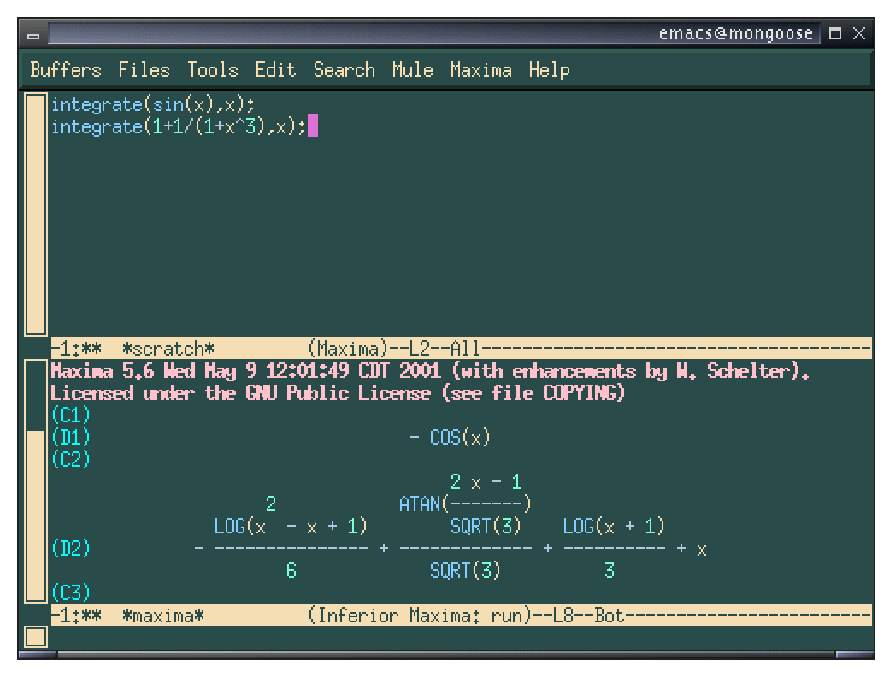
\includegraphics{images/emacsmaximamodeshot} 
\caption{Maxima-mode} 
\end{figure}

\noindent
When something is sent to Maxima, a buffer running an inferior Maxima 
process will appear.  It can also be made to appear by using the command
\texttt{C-c C-p}.
If an argument is given to a command to send information to Maxima,
the region (buffer, line, form) will first be checked to make sure
the parentheses are balanced.
The Maxima process can be killed, after asking for confirmation 
with \texttt{C-cC-k}.  To kill without confirmation, give \texttt{C-cC-k}
an argument.

By default, a newline will be indented to the same level as the 
previous line, with an additional space added for open parentheses.
A tab will add extra spaces, as determined by the value of the 
variable \texttt{maxima-indent-amount}.  By default, this is 2.
The behaviour of newline and indent can be changed by the command 
\texttt{M-x maxima-change-newline-style}.  The possibilities are:
\begin{description}
\item[Basic] A newline will have no indentation, and indentation
               must be added with tabs.
\item[Standard]      As above.
\item[Perhaps smart] Tries to guess an appropriate indentation, based on
               open parentheses, "do" loops, etc.
               A newline will re-indent the current line, then indent
               the new line an appropriate amount.
\end{description}
The default can be set by setting the value of the variable 
\texttt{maxima-newline-style} to either \texttt{'basic}, 
\texttt{'standard} or \texttt{'perhaps-smart}.
In all cases, \texttt{M-x maxima-untab} will remove a level of indentation.

\subsection{Enhanced Terminal Mode}

For those just want a better terminal session, you can run a regular terminal
style session in Emacs.  This gives you everything the 
terminal interface does, plus syntax highlighting, plus more flexibility when
editing your commands.  If you already have a copy of Emacs open, you can start
up the Maxima buffer by typing \verb@ M-x maxima @.  If you do not have Emacs
running, a shortcut is to start emacs using the following command: \verb@ emacs -f maxima @.  

\begin{figure}
\centering 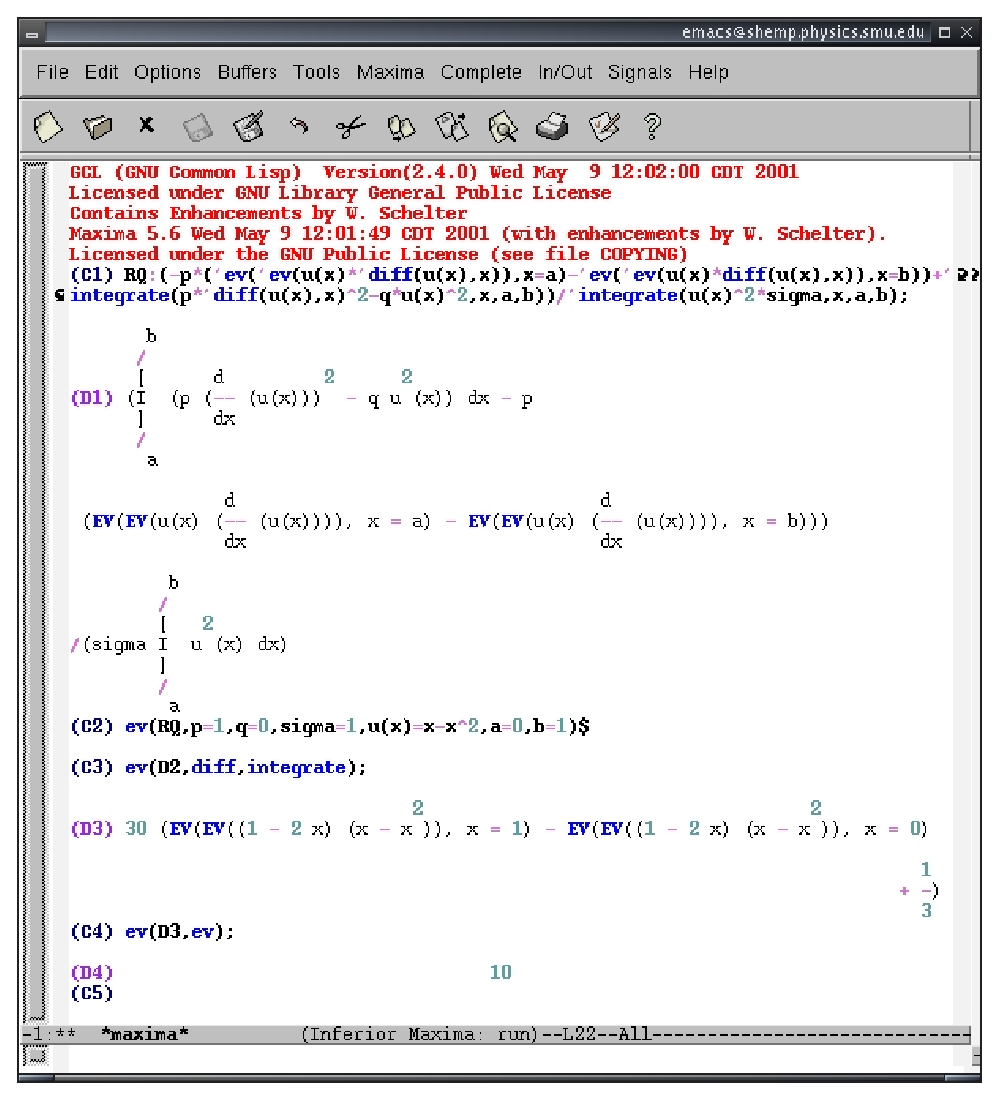
\includegraphics{images/emacsshot}
\caption{Enhanced Terminal Mode}
\end{figure}

In the Maxima process buffer,
return will check the line for balanced parentheses, and send line as input.
Control return will send the line as input without checking for balanced
parentheses.  The following commands are also available.

\smallskip

\begin{tabular}{p{\firstcol}p{\secondcol}}
\texttt{M-TAB} & Complete the Maxima symbol as much as possible, providing
     a completion buffer if there is more than one possible completion.\\
\texttt{C-TAB} & Cycle through possible completions.\\
\texttt{C-M-TAB} & Complete the input line, based on previous input lines.\\
\texttt{C-c C-d} & Get help on a Maxima topic.\\
\texttt{C-c C-m} & Bring up the Maxima info manual.\\
\texttt{C-cC-k} & Kill the process and the buffer, after asking for
  confirmation.  To kill without confirmation, give \texttt{C-cC-k} an
  argument.\\
\texttt{M-p} & Bring the previous input to the current prompt.\\
\texttt{M-n} & Bring the next input to the prompt.\\
\texttt{M-r} & Bring the previous input matching
  a regular expression to the prompt.\\
\texttt{M-s} & Bring the next input matching
  a regular expression to the prompt.
\end{tabular}


\subsection{Emaxima Mode}

Emaxima is a major mode for Emacs that allows the user to insert Maxima
sessions and code in a \LaTeX{} document.  It is based on Dan Dill's
\TeX{}/\textit{Mathematica} package\footnote{\TeX/\textit{Mathematica} is
available from \url{ftp://chem.bu.edu/pub/tex-mathematica-2.0}.}, and
uses a modified version of William Schelter's \texttt{maxima.el}.
Emaxima is an extension of the
\LaTeX{} mode provided by AUC\TeX{}\footnote{This can be configured so
that Emaxima extends the standard \TeX{} mode provided by Emacs, or just
text mode.}, and so has the \LaTeX{} mode commands available.  The
resulting document can be processed by \LaTeX{}; this requires putting 
\begin{verbatim}
\usepackage{emaxima}
\end{verbatim}
\noindent
in the preamble.

This is in no sense a graphical environment, and the user will not see
the benefits of any TeX formatting in real time.  This mode is most 
useful to those who are accustomed to writing documents in LaTeX,
and would like to include Maxima sessions in them.  This manual itself
is a good example of Emaxima in action.

\subsubsection{Cells}

The basic unit of Maxima code in Emaxima is a \textbf{cell}.  A cell
consists of text between the delimiters
\begin{verbatim}
\beginmaxima
\end{verbatim}
\noindent
and
\begin{verbatim}
\endmaxima
\end{verbatim}
\noindent
A cell can be created by typing \texttt{C-c C-o}.  (The \texttt{C-o} in this
case stands for \textbf{o}pening a cell.)  The delimiters will then be
placed in the buffer, and the point will be placed between them.

When working with several cells, you can jump between them by using
\texttt{C-c +} to go to the next cell and \texttt{C-c -} to go to the
previous cell.

\begin{figure}

\centering 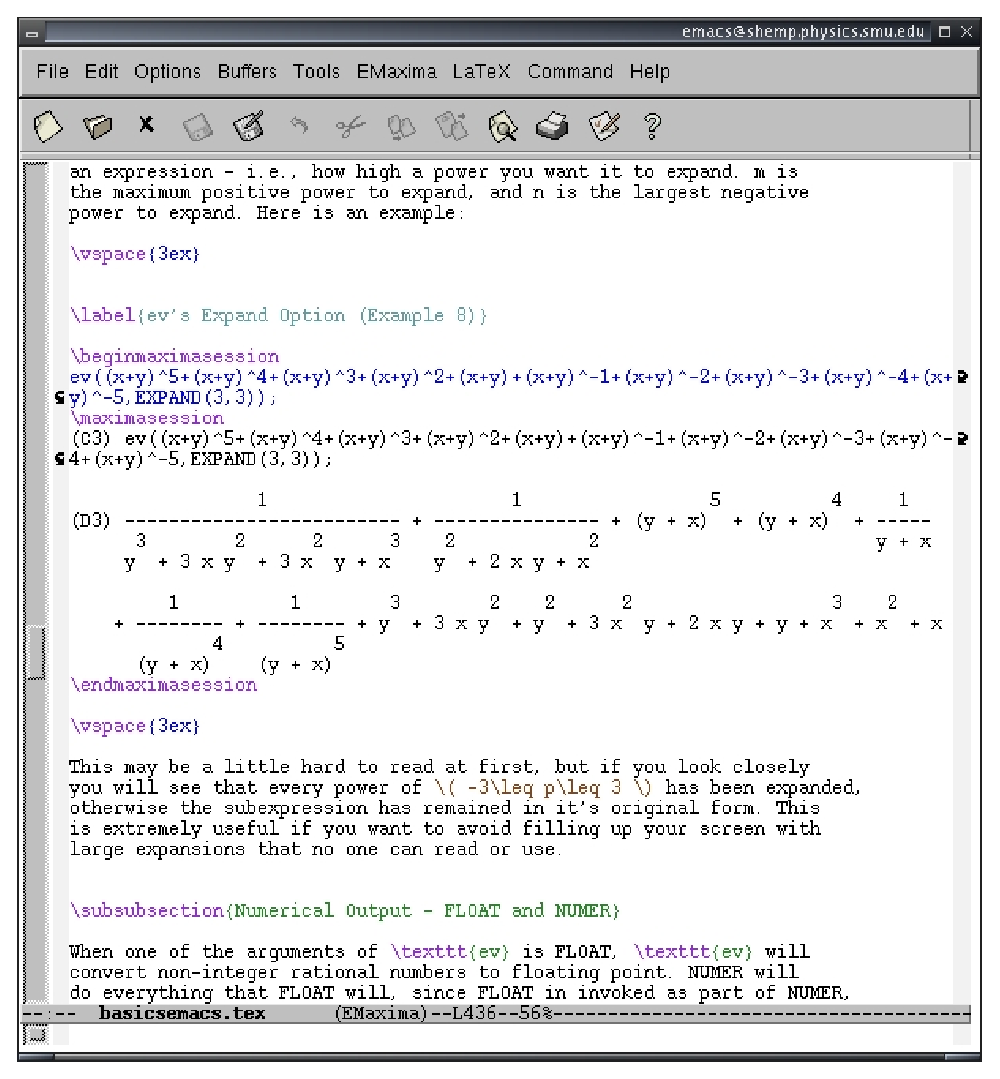
\includegraphics{images/emaximashot} \par
\caption{An Emaxima Session}

\end{figure}

\subsubsection{Evaluating cells}

\noindent
To evaluate the contents of a cell, the command
\texttt{C-cC-uc} (\texttt{emaxima-update-cell})\footnote{Sending the
  cells contents to a Maxima process and returning the results is
  called \textbf{updating} the cell, the prefix 
\texttt{C-c C-u} will be used to update cells in different ways.} 
will send the contents
of the cell to a Maxima process (if there is no Maxima process running,
one will be started) and return the results to the cell,
separated from the input by the marker
\begin{verbatim}
\maximaoutput
\end{verbatim}
\noindent
To differentiate
$sin(x^2)$, for example, type 
\texttt{diff(sin(x\^{}2),x);} in a cell:
\begin{verbatim}
\beginmaxima
diff(sin(x^2),x);
\endmaxima
\end{verbatim}
\noindent
After typing \texttt{C-c C-u c}, it will look like
\begin{verbatim}
\beginmaxima
diff(sin(x^2),x);
\maximaoutput
                                           2
                                  2 x COS(x )
\endmaxima
\end{verbatim}
\noindent
To delete the output and return the cell to its original form, you can
use the command \texttt{C-c C-d}.
If the document is to be \TeX{}ed, the above cell will look like:
\beginmaxima
diff(sin(x^2),x);
\endmaxima
and the cell with output will look like:
\beginmaxima
diff(sin(x^2),x);
\maximaoutput
                                           2
                                  2 x COS(x )
\endmaxima

Emaxima mode can take advantage of the fact that Maxima can give its
output in \LaTeX{} form.  The command \texttt{C-c C-u C}
works the same as \texttt{C-c C-u c}, except now the output is in \LaTeX{}
form, ready to be formatted by \LaTeX{}.  In general, if 
\texttt{C-c C-u }\textsl{letter} returns Maxima output, then
\texttt{C-c C-u }\textsl{capital letter} will return the output in
\TeX{} form.  The above cell would become
\begin{verbatim}
\beginmaxima
diff(sin(x^2),x);
\maximatexoutput
$$   2\*x\*\cos x^{2} $$
\endmaxima
\end{verbatim}
\noindent
which, when \LaTeX{}ed, would become
\beginmaxima
diff(sin(x^2),x);
\maximatexoutput
$$   2\*x\*\cos x^{2} $$
\endmaxima
\noindent
(Note that whenever a cell is updated, any old output is discarded and
replaced with new output.)  The command \texttt{C-c C-u a} will update all
of the cells in your document, 
stopping at each one to ask if you indeed want it updated.  Given an
argument, \texttt{C-u C-c C-u a}, it will update all of the cells in your
document without asking.  The command \texttt{C-c C-u A} behaves
similarly, except now all the output is returned in \LaTeX{}  form.

\subsubsection{Initialization Cells}

\noindent
It is possible that you want certain cells evaluated separate from the
others; perhaps, for example, you want certain cells evaluated whenever
you open the document.  This can be done using initialization cells.
An initialization cell is delimited by
\begin{verbatim}
\beginmaxima[* Initialization Cell *]
\end{verbatim}
\noindent
and
\begin{verbatim}
\endmaxima
\end{verbatim}
\noindent
The command \texttt{C-c C-t} will turn a cell into
an initialization cell, applying \texttt{C-c C-t} again will turn it
back into a regular cell.  
When \LaTeX{}ed, an initialization cell will look like
\beginmaxima[* Initialization Cell *]
diff(sin(x^2),x);
\endmaxima

Initialization cells behave like regular
cells, except that they can be treated as a group.
To evaluate all initialization cells (without displaying the output in
the document buffer), the
command \texttt{C-c C-u t} will go to each of the
initialization cells and evaluate them.
If you want the output of the initialization cells to be brought back 
to the document buffer,  stopping at each one to see it
you indeed want it updated, then use the command \texttt{C-c C-u i}.
With an argument, \texttt{C-u C-c C-u i}, the
initialization cells will be updated without asking.   The command 
\texttt{C-c C-u I} behaves just like \texttt{C-c C-u i},
except that the output is returned in \TeX{} form.

\subsubsection{Referencing Other Cells}

\noindent
Instead of Maxima code, a cell can contain a reference to another cell,
and when the original cell is sent to Maxima, the reference is replaced
by the referenced cell's contents (but only in the Maxima process
buffer, the cell's 
content in the document's buffer is not changed).  In order to do
this, the original cell must be marked by having a label of the form
\texttt{<}\textsl{filename}\texttt{:}\textsl{cell label}\texttt{>}.
(The reason for the \textsl{filename} will become apparent later, and
\textsl{cell label} is optional for the referencing cell.)
The referenced cell must also be labeled, with the same
\textsl{filename} but a unique \textsl{cell label}.  To reference the
other cell, the original cell need only contain the marker for the
referenced cell.  For example, given cell 1:
\begin{verbatim}
\beginmaxima<filename:optional>
<filename:definef>
diff(f(x),x);
\endmaxima
\end{verbatim}
\noindent
and cell 2:
\begin{verbatim}
\beginmaxima<filename:definef>
f(x):=sin(x^2);
\endmaxima
\end{verbatim}
\noindent
then the result of updating cell 1 (\texttt{C-c C-u c}) will be:
\begin{verbatim}
\beginmaxima<filename:optional>
<filename:definef>
diff(f(x),x);
\maximaoutput
                                             2
                                f(x) := SIN(x )
                                           2
                                  2 x COS(x )
\endmaxima
\end{verbatim}
\noindent
When \LaTeX{}ed, the top line will contain a copy of the marker.

\beginmaxima<filename:optional>
<filename:definef>
diff(f(x),x);
\maximaoutput
                                             2
                                f(x) := SIN(x )
                                           2
                                  2 x COS(x )
\endmaxima

A cell can contain more than one reference, and referenced cells can
themselves contain references.  

To aid in labelling the cells, the command \texttt{C-c C-x}
will prompt for a label name and label the
cell.  To aid in calling references, the command \texttt{C-c C-TAB}
can be used for completing the
the \textsl{filename} and \textsl{cell label} parts of a reference, 
based on the current labels.  
Another option is to set the Emacs variable
\texttt{emaxima-abbreviations-allowed} to \texttt{t}, say, by putting
the line
\begin{verbatim}
(setq emaxima-abbreviations-allowed t)
\end{verbatim}
\noindent
in your \texttt{.emacs} file.  This will allow the \textsl{filename}
and \textsl{cell label} parts of a reference to be abbreviated by enough
of a prefix to uniquely identify it, followed by ellipses
\texttt{...}
For example, if there are cells labelled
\begin{verbatim}
<filename:long description>
<filename:lengthy description>
\end{verbatim}
\noindent
Then the reference
\begin{verbatim}
<...:le...>
\end{verbatim}
\noindent
will suffice to refer to the second label above.

If you want the references in a cell to be replaced by the actual
code, the command \texttt{C-c @} will expand all the
references and put the code into a separate buffer (so it will not
affect the original document).

\subsubsection{WEB}

\noindent
The reason for the ability to reference other cells is so that you can
write what Donald Knuth calls literate programs.  The idea is that the
program is written in a form natural to the author rather than natural
to the computer.  (Another aspect of Knuth's system is that the code
is carefully documented, hence the name ``literate programming'', but
that is done naturally in Emaxima.)  Knuth called his original
literate programming tool \texttt{WEB}, since, as he puts it,
``the structure of a software program may be thought of as a web that
is made up of many interconnected pieces.''  
Emaxima's ability in this respect is taken directly from
\TeX{}/\textit{Mathematica}, and is ultimately based on
\texttt{WEB}. To create a 
program, the ``base cell'' or ``package cell'' should contain 
a label of the form \texttt{<}\textsl{filename}\texttt{:>} 
(no cell label), and can
contain references of the form 
\texttt{<}\textsl{filename}\texttt{:}\textsl{part}\texttt{>}
(same file name as the base cell).  

As a simple (and rather silly) example, suppose we want to create a
program to sum the first $n$ squares.  We could start:
\begin{verbatim}
\beginmaxima<squaresum.max:>
squaresum(n) := (
  <squaresum.max:makelist>
  <squaresum.max:squarelist>
  <squaresum.max:addlist>
  );        
\endmaxima
\end{verbatim}
\noindent
We would then need cells
\begin{verbatim}
\beginmaxima<squaresum.max:makelist>,
L:makelist(k,k,1,n),
\endmaxima

\beginmaxima<squaresum.max:squarelist>
<squaresum.max:definesquare>
L:map(square,L),
\endmaxima

\beginmaxima<squaresum.max:addlist>
lsum(k,k,L)
\endmaxima
\end{verbatim}
\noindent
and then we would also need:
\begin{verbatim}
\beginmaxima<squaresum.max:definesquare>
square(k) := k^2,
\endmaxima
\end{verbatim}
\noindent
When \TeX{}ed, the header of the cell will say that it determines the
file \texttt{squaresum.mu}.  
\beginmaxima<squaresum.max:>
squaresum(n) := (
  <squaresum.max:makelist>
  <squaresum.max:squarelist>
  <squaresum.max:addlist>
  );        
\endmaxima

The command 
\texttt{C-u C-c @} will put all the pieces
together in the file it determines.  The resulting file, in this case,
will be \texttt{squaresum.max} and will look like:
\begin{verbatim}
squaresum(n) := (
  L:makelist(k,k,1,n),
  square(k) := k^2,
  L:map(square,L),
  lsum(k,k,L)
  );        
\end{verbatim}
\noindent
(Although the idea is that only the computer need look at this file.)

\subsubsection{Other types of cells}

\noindent
When a cell is \TeX{}ed, the input and output are kept separate.  To
have the results look like a Maxima session, there are, in addition to
the standard cells, special cells called \emph{session cells}.   A
session cell is delimited by
\begin{verbatim}
\beginmaximasession
\end{verbatim}
\noindent
and
\begin{verbatim}
\endmaximasession
\end{verbatim}
\noindent
The command \texttt{C-c C-p} will create a session cell.  When a
session cell is updated, the output will be marked off with
\verb+\maximasession+, and will contain both the input and the output,
with the Maxima prompts.  For example, if the session cell
\begin{verbatim}
\beginmaximasession
diff(sin(x),x);
int(cos(x),x);
\endmaximasession
\end{verbatim}
\noindent
were updated, the result would look like
\begin{verbatim}
\beginmaximasession
diff(sin(x),x);
integrate(cos(x),x);
\maximasession
(C1)diff(sin(x),x);

(D1)                                COS(x)
(C2)integrate(cos(x),x);

(D2)                                SIN(x)
\endmaximasession
\end{verbatim}
\noindent
which, when \TeX{}ed, would look like
\beginmaximasession
diff(sin(x),x);
integrate(cos(x),x);
\maximasession
(C1)diff(sin(x),x);

(D1)                                COS(x)
(C2)integrate(cos(x),x);

(D2)                                SIN(x)
\endmaximasession
\noindent
If it is updated in \TeX{} form, it will look like
\begin{verbatim}
\beginmaximasession
diff(sin(x),x);
integrate(cos(x),x);
\maximatexsession
\C1.  diff(sin(x),x); \\
\D1.   \cos x \\
\C2.  integrate(cos(x),x); \\
\D2.   \sin x \\
\endmaximasession
\end{verbatim}
\noindent
which, when \TeX{}ed, will look like
\beginmaximasession
diff(sin(x),x);
integrate(cos(x),x);
\maximatexsession
\C1.  diff(sin(x),x); \\
\D1.   \cos x \\
\C2.  integrate(cos(x),x); \\
\D2.   \sin x \\
\endmaximasession

For particularly long output lines inside the \verb+\maximatexsession+
part of a session cell, the command \verb+\DD+ will typeset anything
between the command and \verb+\\+.  Unfortunately, to take advantage
of this, the output has to be broken up by hand.
If a session cell has not been updated, or has no output for some
other reason, it will not appear when the document is \TeX{}ed.

There is one other type of cell, a \emph{noshow cell}, which can be
used to send Maxima a command, but won't appear in the \TeX{}ed
output. A noshow cell can be created with \texttt{C-c C-n}, and will
be delimited by
\begin{verbatim}
\beginmaximanoshow
\end{verbatim}
\noindent
and
\begin{verbatim}
\endmaximanoshow
\end{verbatim}

Session cells and noshow cells cannot be initialization cells or part of
packages.\footnote{That could be changed, but I don't know why it'd be
useful.} 

If the command to create one type of cell is called while inside
another type of cell, the type of cell will be changed.  So, for
example, the command \texttt{C-c C-p} from inside the cell
\begin{verbatim}
\beginmaxima
diff(x*sin(x),x);
\endmaxima
\end{verbatim}
\noindent
will result in
\begin{verbatim}
\beginmaximasession
diff(x*sin(x),x);
\endmaximasession
\end{verbatim}
\noindent
If a standard cell is an initialization cell or a package part, its
type cannot be changed.


\subsubsection{Miscellaneous}

\noindent
Some Maxima commands can be used even outside of cells.  The command 
\texttt{C-c C-u l} send the current line to a
Maxima process, comment out the current line, and insert the Maxima
output in the current buffer.  The command 
\texttt{C-c C-u L} will do the same, but
return the result in \LaTeX{} form.

The command \texttt{C-c C-h} will provide
information on a prompted for function (like Maxima's \texttt{describe}), 
and  \texttt{C-c C-i} will give the Maxima info manual.

Finally, the Maxima process can be killed with \texttt{C-c C-k}.

\subsubsection{Customizing EMaxima}

\noindent
There are a few things that you can do to customize Emaxima.  

By default, Emaxima is an extension of AUC\TeX{} mode.  This can be
changed by changing the variable \texttt{emaxima-use-tex}.  The possible
values are \texttt{'auctex}, \texttt{'tex} and \texttt{nil}.  Setting
\texttt{emaxima-use-tex} (the default) to \texttt{'auctex} will make Emaxima
an extension of AUC\TeX{}, setting it to \texttt{'tex} will make Emaxima an
extension of Emacs's default \TeX{} mode, and setting
\texttt{emaxima-use-tex} to \texttt{nil} will make Emaxima an extension of
text-mode.  So, for example, putting 
\begin{verbatim}
(setq emaxima-use-tex nil)
\end{verbatim}
\noindent
in your \texttt{.emacs} file will make Emaxima default to an extension of
text mode. 

Whether or not the dots (\dots{}) abbreviation is allowed in cell
references is controlled by the elisp variable
\texttt{emaxima-abbreviations-allowed}, which is set to \texttt{t} by
default.  Setting this to \texttt{nil} will disallow the abbreviations,
but will speed up package assembly.

The \LaTeX{}ed output can also be configured in a couple of ways.
The lines that appear around cells when the document is \TeX{}ed can be
turned off with the command (in the \LaTeX{} document)
\begin{verbatim}
\maximalinesfalse
\end{verbatim}
\noindent
They can be turned back on with the command
\begin{verbatim}
\maximalinestrue
\end{verbatim}
\noindent

The fonts used to display the Maxima input and output in a cell are by
default \texttt{cmtt10}.  They can be changed, seperately, by changing the
\TeX{} values of \verb+\maximainputfont+ and \verb+\maximaoutputfont+.
So, for example, to use \texttt{cmtt12} as the input font, use the command
\begin{verbatim}
\font\maximainputfont = cmtt12
\end{verbatim}
\noindent
The spacing in the cells can be controlled by changing the \TeX{}
variables \verb+\maximainputbaselineskip+ and
\verb+\maximaoutputbaselineskip+, and so to increase the space between
the lines of the output, the command
\begin{verbatim}
\maximaoutputbaselineskip = 14pt
\end{verbatim}
\noindent
could be used.
The amount of space that appears before a cell can be changed by changing
the value of \verb+\premaximaspace+ (by default, 0pt), and that after
a cell can be changed by changing the value of \verb+\postmaximaspace+
(by default, 1.5 ex).
 
Session cells can be configured similarly.  
Lines can be placed around a Maxima session with the command
\begin{verbatim}
\maximasessionlinestrue
\end{verbatim}
\noindent
and they can be turned back off with
\begin{verbatim}
\maximasessionlinesfalse
\end{verbatim}
\noindent
The font can be changed by changing the value of
\verb+\maximasessionfont+.  The color of the prompts when the session
is in \TeX{} form is controlled by \\
\verb+\maximapromptcolor+, by
default red, the colors of the input lines and output lines are
controlled by \verb+\maximainputcolor+ and \verb+\maximaoutputcolor+,
respectively. So the command
\begin{verbatim}
\def\maximainputcolor{green}
\end{verbatim}
\noindent
would make the input in a \TeX{}ed session green.  
The session can be \TeX{}ed without the colors by using the command
\verb+\maximasessionnocolor+.
The baselineskip is
set by \verb+\maximasessionbaselineskip+ for normal session cells, and
by \verb+\maixmatexsessionbaselineskip+ for \TeX{} sessions.  The
amount of space that appears before a session cell can be changed by
changing the value of \verb+\premaximasessionspace+ (by default, 0pt),
and that after a cell can be changed by changing the value of
\verb+\postmaximasessionspace+ (by default, 1.5 ex).

\subsubsection{Emaxima mode commands}

\noindent
\begin{tabular}{p{\firstcol}p{\secondcol}}
\hline
\textbf{Key} & \textbf{Description}\\
\hline
\texttt{C-c C-o} & Create a (standard) cell.\\
\texttt{C-c C-p} & Create a session cell.\\
\texttt{C-c C-n} & Create a noshow cell.\\
\texttt{C-c +} & Go the the next cell.\\
\texttt{C-c -} & Go to the previous cell.\\
\texttt{C-c C-u a} & 
Update all of the cells.  With an argument, don't ask before updating.\\
\texttt{C-c C-u A}
& Update all of the cells in \TeX{} form. With an argument don't ask
before updating.\\
\texttt{C-c C-u t}
& Evaluate all of the initialization cells.\\
\texttt{C-c C-u i}
& Update all of the initialization cells.  With an argument, don't
ask before updating.\\
\texttt{C-c C-u I}
& Update all of the initialization cells in \TeX{} form.  With an
argument, don't ask before updating.\\
\texttt{C-c C-u s}
& Update all of the session cells in \TeX{} form.  With an
argument, don't ask before updating.\\
\texttt{C-c C-k}
& Kill the current Maxima core - this will lose all data entered
into the maxima system up until this point by other cells.
\end{tabular}

\smallskip

\noindent
\textbf{Commands only available in cells.}

\smallskip

\noindent
\begin{tabular}{p{\firstcol}p{\secondcol}}
\hline
\textbf{Key} & \textbf{Description}\\
\hline
\texttt{C-c C-v}
%& \texttt{emaxima-send-cell}
& Send the current cell to the Maxima process.\\
\texttt{C-c C-u c}
%& \texttt{emaxima-update-cell}
& Update the current cell.\\
\texttt{C-c C-u C}
%& \texttt{emaxima-tex-update-cell}
& Update the current cell in \TeX{} form.\\
\texttt{C-c C-d}
%& \texttt{emaxima-delete-output}
& Delete the output from the current cell.\\
\texttt{C-c C-t}
%& \texttt{emaxima-toggle-init}
& Toggle whether or not the current cell is an initialization cell.\\
\texttt{C-c C-x}
%& \texttt{emaxima-package-part}
& Insert a heading for the cell indicating that it's part of a
package. \\
\texttt{C-c @}
%& \texttt{emaxima-assemble}
& Assemble the references contained in the cell.  With an argument,
assemble the package that the cell defines.\\
\texttt{C-c C-\texttt{TAB}}
%& \texttt{emaxima-insert-complete-name}
& Complete a reference within a cell.
\end{tabular}

\smallskip

\noindent
\textbf{Commands only available outside of cells.}

\smallskip

\noindent
\begin{tabular}{p{\firstcol}p{\secondcol}}
\hline
\textbf{Key} & \textbf{Description}\\
\hline
\texttt{C-c C-u l}
%& \texttt{emaxima-replace-line}
& Send the current line to Maxima, and replace the line with the
Maxima output.\\
\texttt{C-c C-u L}
%& \texttt{emaxima-replace-line-with-tex}
& Send the current line to Maxima, and replace the line with the
Maxima output in \TeX{} form.
\end{tabular}

\subsubsection{AUC\TeX{} commands}

\smallskip

\noindent
\textbf{Inserting commands}

\smallskip

\noindent
\begin{tabular}{p{\firstcol}p{\secondcol}}
\hline
\textbf{Key} & \textbf{Description}\\
\hline
\texttt{C-c C-e}
& Insert an environment.\\
\texttt{C-c C-s}
& Insert a section.\\
\texttt{C-c ]}
& Close an environment.\\
\texttt{C-c C-j}
& Insert an item into a list.\\
\texttt{"}
& Smart quote.\\
\texttt{\$}
& Smart dollar sign.\\
\texttt{C-c @}
& Insert double brace.\\
\texttt{C-c C-m}
& Insert \TeX{} macro.\\
\texttt{M-TAB}
& Complete \TeX{} macro.\\
\end{tabular}

\smallskip

\noindent
\textbf{Formatting}

\smallskip

\noindent
\begin{tabular}{p{\firstcol}p{\secondcol}}
\hline
\textbf{Key} & \textbf{Description}\\
\hline
\texttt{C-c C-q C-r}
& Format region.\\
\texttt{C-c C-q C-s}
& Format section.\\
\texttt{C-c C-q C-e}
& Format environment.\\
\texttt{C-c .}
& Mark an environment.\\
\texttt{C-c *}
& Mark a section.
\end{tabular}

\smallskip

\noindent
\textbf{Commenting}

\smallskip

\noindent
\begin{tabular}{p{\firstcol}p{\secondcol}}
\hline
\textbf{Key} & \textbf{Description}\\
\hline
\texttt{C-c ;}
& Comment a region.\\
\texttt{C-u C-c ;}
& Uncomment a region.\\
\texttt{C-c \%}
& Comment a paragraph.\\
\texttt{C-u C-c \%}
& Uncomment a paragraph.
\end{tabular}

\smallskip

\noindent
\textbf{Font selection}

\smallskip

\noindent
\begin{tabular}{p{\firstcol}p{\secondcol}}
\hline
\textbf{Key} & \textbf{Description}\\
\hline
\texttt{C-c C-f C-b}
& Bold.\\
\texttt{C-c C-f C-i}
& Italics.\\
\texttt{C-c C-f C-r}
& Roman.\\
\texttt{C-c C-f C-e}
& Emphasized.\\
\texttt{C-c C-f C-t}
& Typewriter.\\
\texttt{C-c C-f C-s}
& Slanted.\\
\texttt{C-c C-f C-d}
& Delete font.\\
\texttt{C-u C-c C-f}
& Change font.
\end{tabular}

\smallskip

\noindent
\textbf{Running \TeX{}}

\smallskip

\noindent
(Commands: \texttt{TeX}, \texttt{TeX Interactive}, \texttt{LaTeX},
\texttt{LaTeX Interactive}, \texttt{SliTeX}, \texttt{View},
\texttt{Print}, \texttt{BibTeX}, \texttt{Index}, \texttt{Check},
\texttt{File}, \texttt{Spell}.)

\smallskip

\noindent
\begin{tabular}{p{\firstcol}p{\secondcol}}
\hline
\textbf{Key} & \textbf{Description}\\
\hline
\texttt{C-c C-c}
& Run a command on the master file.\\
\texttt{C-c C-r}
& Run a command on the current region.\\
\texttt{C-c C-b}
& Run a command on the buffer.\\
\texttt{C-c `}
& Go to the next error.\\
\texttt{C-c C-k}
& Kill the \TeX{} process.\\
\texttt{C-c C-l}
& Center the output buffer.\\
\texttt{C-c C-\^{}}
& Switch to the master file.\\
\texttt{C-c C-w}
& Toggle debug of overful boxes.\\
\end{tabular}

\section{Xmaxima}
~

{\centering 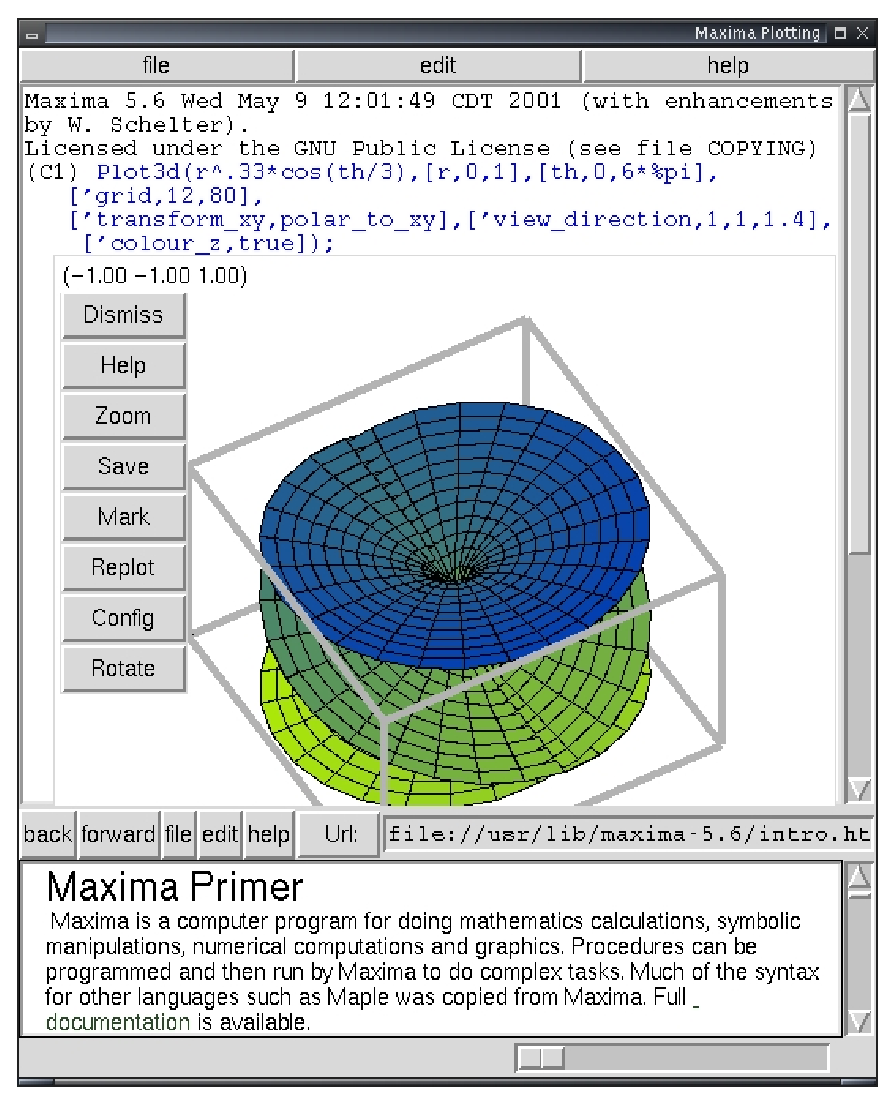
\includegraphics{images/xmaxima} \par}

~

Xmaxima is a new development in the lifetime of Maxima. It is based
on Tcl/Tk, and has the nifty feature of in-line plotting when using
the default plotting routine. No version earlier than ? has this interface,
so if you aren't using the new versions you won't have this included
in your default package. This is probably where most people will start
learning Maxima, and it is not a bad place to start. You avoid the
earlier mentioned limitations of the vanilla terminal, and avoid having
to master the setup for Emacs. In order to start this interface simply
type xmaxima in a terminal. From there, you should get what looks
like the terminal interface in a Tk window, with an introductory html
document below it. There is also a pull down menu system. For Windows
users, this will more than likely be the default choice. Symaxx and
\TeX{}macs are Unix only.

\section{Symaxx}

In the words of its creator Markus Nentwig ``Symaxx provides those 5\% of features,
that are needed to do 95\% of your work.'' Perhaps the best description
of its display is that of a mathematical flowchart - it indicates relationships
between cells with arrows, and allows free placement of expressions on a
canvas.  It is more graphical than
any of the other Maxima interfaces, and although input is still ascii
based the output is formatted. It is based on Perl and Tk, both of
which are required to run it. This interface tends, at least in the
experience of this author, to be a bit resource intensive, but allows
some page formatting possibilities which make it a very interesting
program. We will show you some of its features here, and if you decide to use
this interfacethe Symaxx manual is a highly recommended
read.

~

{\centering 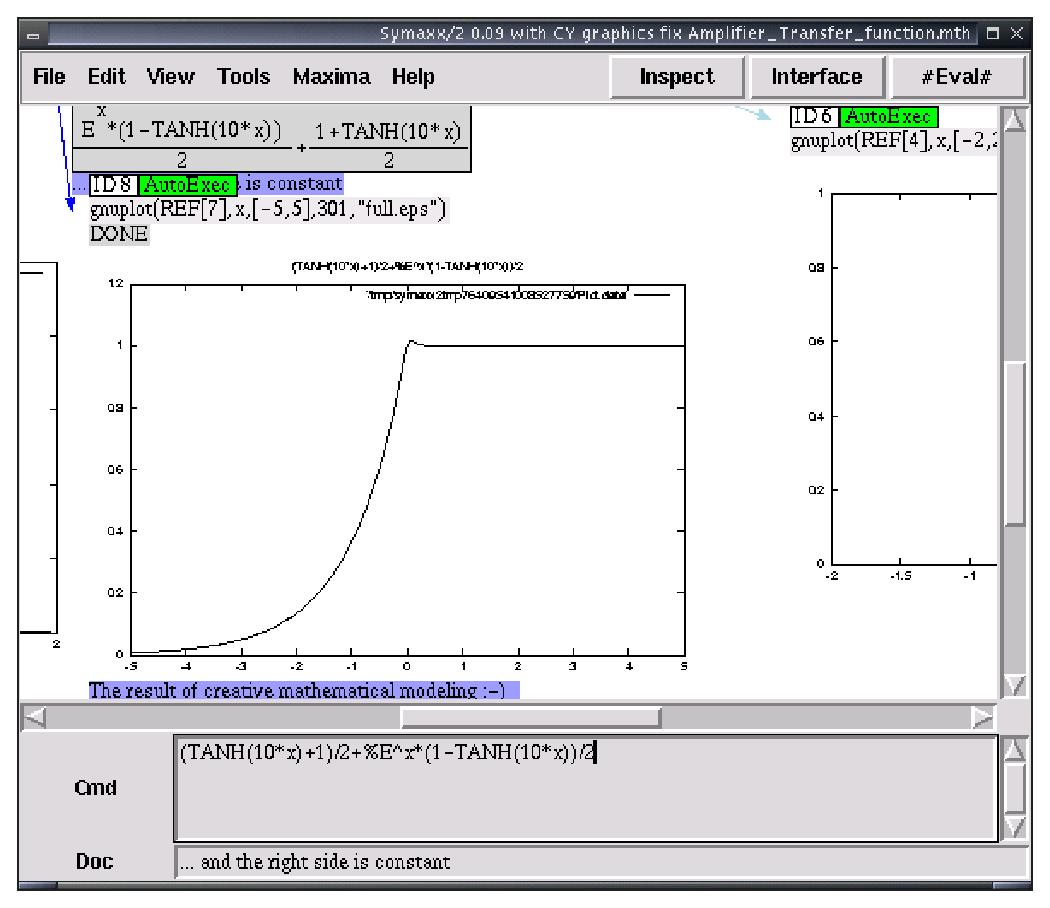
\includegraphics{images/symaxx} \par}

~
 
Symaxx uses a fairly basic display format - each unit of mathematical input
and output is labeled with an ID number, which one can use to refer to 
that particular unit elsewhere in your document.  There are three levels to
each unit - the input box, which displays the command input into Maxima,
the output box, which displays the results, and the documentation box,
where you can record information and descriptions which are not intended
to be evaluated.  This may take a little getting used to - pressing return
once you are done creating the input expression doesn't evaluate it, but only
sends it to the formatter used by Symaxx to create a graphical representation
of the input.  To send the command to Maxima, you press the evaluate button.

For graphing purposes, Symaxx is able to embed gnuplot figures.  Also included
in its abilities are the ability to use TeX to display output, manipulate
units, and export to postscript files.  Here is a sample output showing
these abilities in action:

~

{\centering 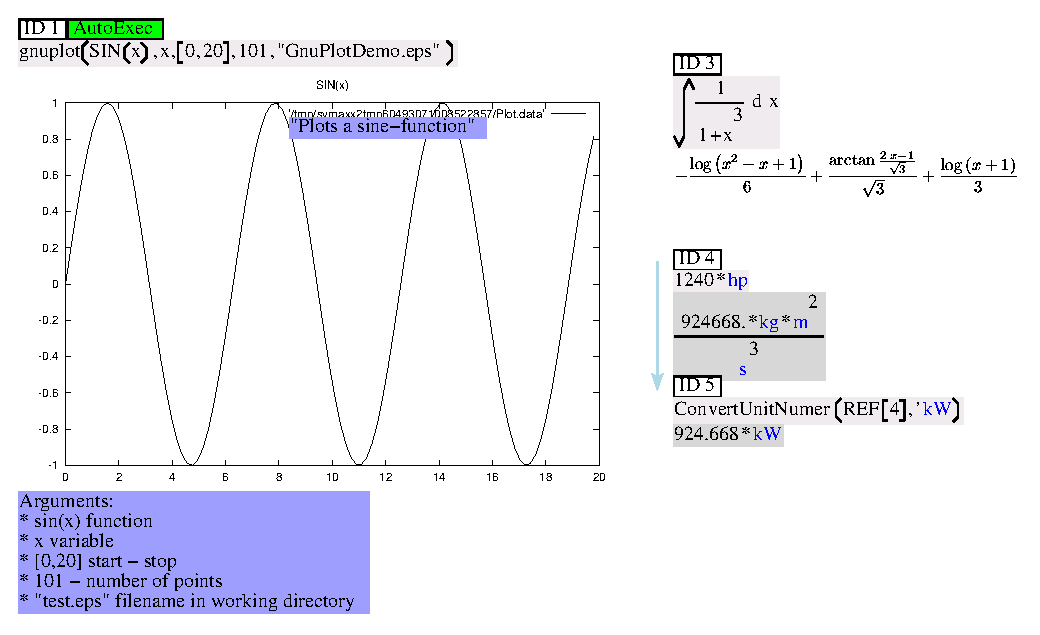
\includegraphics{images/symaxxoutput} \par}

~

(Add to
troubleshooting tips:  Some versions
of Symaxx seem to have trouble interacting with some versions of netpbm - if Symaxx
should fail to display graphs, try this solution:
~
get solution from Symaxx discussion forum
~
)

In order to utilize the full abilities of Symaxx, you must have a fair bit of
supporting software installed.  There is Maxima itself, of course, and then there
are the following:
\begin{itemize}
\item Perl
\item Tk800.022
\item netpbm
\item \TeX{} for advanced output formatting 
\end{itemize}

Here are some basic install instructions. We will assume here you need to install
Tk800.022 and Symaxx, having already installed the others earlier.  If you haven't
they are readily available on most Linux distributions.

\begin{verbatim}
user$ tar -xvzf Tk800.022.tar.gz 
user$ cd Tk800.022

If you have root access, do the following:

user$ perl Makefile.PL
user$ make
user$ make test (optional)
user$ su
Password:
root$ make install

if you don't have root access, use

user$ perl Makefile.PL LIB=/home/(place to install) or
user$ perl Makefile.PL PREFIX=/home/(place to install).
user$ make; make install
\end{verbatim}

Find the location of the folder `Tk' in the folder you gave as argument to LIB or
PREFIX. Now you'll have to change the first line in `symaxx' and `Symaxx2/Watchdog'
to include the Tk library. Append a
\verb@-I /home/(where you installed Tk)/@ \verb@(The folder that contains Tk)@
as in
\verb@ #!/usr/bin/perl -w -I /home/somewhere/ @

Then simply decompress Symaxx in the directory of your choice. If perl is not in /usr/bin, you'll have to change the first line of the files `symaxx'
and `Symaxx2/Watchdog' to the location on your system, as found by `whereis
perl'.

\section{\TeX{}macs}

\TeX{}macs is a new WYSIWYG scientific editor, and it has the ability
to interface with many computer algebra systems, including Maxima.
This program takes advantage of the \TeX{} output Maxima can produce
to format it's output. To launch Maxima inside of \TeX{}macs you go
up to the menu and select Insert -> sessions -> maxima. Then things
work like they do in xmaxima or Emacs. This is probably the most visually
appealing way to run Maxima.  You can insert a maxima session in TeXmacs by
selecting Insert->session->maxima from the menu.  From there the interface
will feel pretty much like a regular terminal.

~

\begin{figure}
\centering 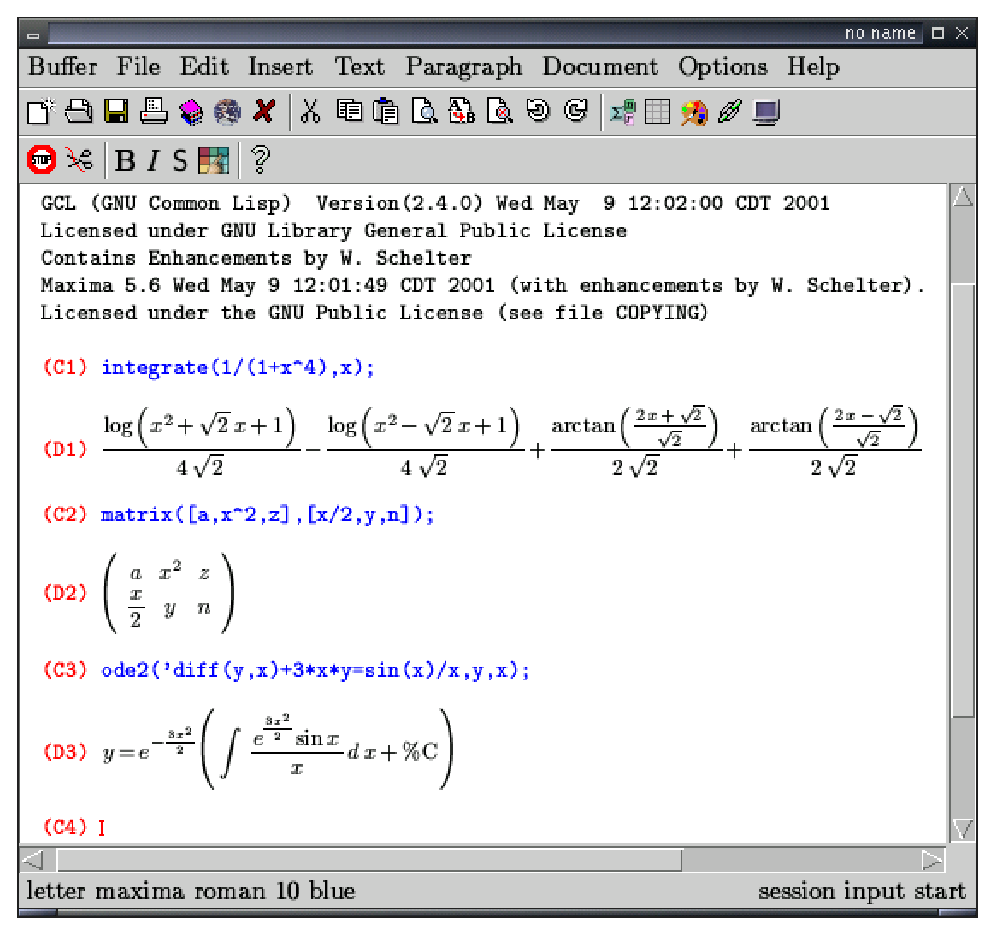
\includegraphics{images/texmacs} 
\caption{TeXmacs with a Maxima Session} 
\end{figure}
